\chapter{Graph Ramsey Theory}\label{chap:graph_ramsey}
This chapter introduces graph Ramsey theory, and is based upon \cite{rt} and \cite{rtoi}[Chapter 1]. We will start by introducing the concept of a coloring and some related concepts.
\begin{definition}
	Let $A$ be a set, an \textit{$r$-coloring} on $A$ is a function $\chi: A \to C$ where $C$ is the set of \textit{colors} and $\abs{C} = r$. Let $a \in A$ if $\chi(a) = c$, then $a$ is said to be \textit{colored} $c$ by $\chi$. The subset $B \subseteq A$ is called \textit{monochromatic} if $\abs{\chi(B)} = 1$. Finally if $\mathcal{F} \subseteq \mathcal{P}(A)$ we say that $\chi$ \textit{admits} a monochromatic instance in $\mathcal{F}$ is there exists some monochromatic $B \in \mathcal{F}$.
\end{definition}
In order to visually illustrate the ideas presented through examples we often simply color (this time literally) each object a given color.

\begin{remark}\label{rem:color_sets}
The concrete choice of color set $C$, in our $r$-coloring $\chi: A \to C$, is not really a concern, since given any bijection $\phi$ between $C$ and another color set $C'$ one would obtain a new $r$-coloring $\chi' = \phi \circ \chi$.
Hence for the sake of simplicity we usually pick $C = \left\{c_1, c_2, \ldots, c_{r}\right\}$, unless $r = 2$ or $r = 3$ in which cases we usually let $C = \left\{red, blue\right\}$ or $C = \left\{red, blue, green\right\}$ respectively.
\end{remark}
\begin{remark}\label{rem:correspondence_between_colorings_and_partition}
	Every $r$-coloring $\chi: A \to \left\{c_1, c_2, \ldots, c_{r}\right\}$, corresponds to a partition of $A$ into $r$-subsets, that is the sets $A_{i} = \left\{a \in A \middle| \chi(a) = c_{i}\right\}$ for $i \in [1; r]$, and vice versa. Throughout the project we will use this correspondence, to use what ever framework is deemed most appropriate.
\end{remark}
The following theorem will play a pivotal role, in establishing some of the more elemental results.
\begin{theorem}[Generalized Pigeonhole Principle]\label{thm:gpp}
	Let $m, r \in \mathbb{N}^{+}$ and $A$ be a set such that $\abs{A} \geq m \cdot r$, if $A_1, A_2, \ldots A_r \subseteq A$ such that $A = \bigcup_{i = 1}^{r} A_i$, then there exists an $A_j$ with $\abs{A_j} > m$.
\end{theorem}
\begin{proof}
	Assume for the sake of contradiction that $\abs{A_j} < m$ for all $j = [r]$, then:
	\begin{equation*}
		\abs{A} \leq \sum_{j = 1}^r \abs{A_i} < r \cdot m
	\end{equation*}
	clearly a contradiction.
\end{proof}
We will primarily use the Generalized Pigeonhole Principle (Theorem \ref{thm:gpp}) by using the natural correspondence between partitions and colorings as desribed in Remark \ref{rem:correspondence_between_colorings_and_partition}.

Throughout this section we will primarily be interested in the case where $A$ is the set of edges $E$ of some graph $G$, in which case we will refer to $\chi$ as an \textit{edge coloring} on $G$.
Hence we shall need some basic notions from graph theory. Throughout the rest of this project a graph shall refer to a simple graph, unless otherwise specified. We say that a subgraph $H$ of $G$ is monochromatic, under $\chi$, if every edge in $H$ is colored the same color by $\chi$

\begin{definition}
	Let $G = (V, E)$ be a graph, $G$ is called \textit{complete} if $v, u \in V$ such that $v \neq u$ implies $\left\{v, u\right\} \in E$. A \textit{subgraph} of $G$ is a graph $G' = (V', E')$ such that $V' \subseteq V$ and $E' \subseteq E$. Finally a complete subgraph is called a \textit{clique}.
\end{definition}
\begin{remark}
	Given a graph $G$ we will some times abuse the notation and simply write $V(G)$ to mean the vertex set of $G$ and $E(G)$ to mean the edge set of $G$.
\end{remark}
We often denote a complete graph with $n$ vertices as $K_n^{*}$ or $K_n$. With the conventions that $V(K_n^{*}) = [0; n - 1]$ and $V(K_n) = [1; n]$ that is the sets $\left\{0, 1, \ldots, n - 1\right\}$ and $\left\{1, 2, \ldots, n\right\}$ respectively.

\begin{definition}\label{def:cliques_and_neighbours}
	Let $G = (V, E)$ be a graph and $U \subseteq V$. We denote the subgraph of $G$ consisting of the vertices in $U$ by $G|_U$ that is:
	\begin{equation*}
		G|_U := \left(U, E \cap (U \times U)\right)
	\end{equation*}
	If $\chi: E \to C$ an $r$-edge coloring on $G$, we will define the set:
	\begin{equation*}
		\mathcal{C}_{\chi}(G; \ell) := \left\{ G|_{U} \middle| U \subseteq V, \abs{U}  = \ell \text{ and }  \abs{\chi(E \cap \left(U \times U)\right)} = 1 \right\}
	\end{equation*}
	That is $\mathcal{C}_{\chi}(G; \ell)$ is the set of all monochromatic cliques (under $\chi$) of order $\ell$, note that $\chi$ may be omitted if no confusion is likely to be occur. Additionally we let:
	\begin{equation*}
		\mathcal{N}_{\chi}(v; c) := \left\{u \in V \middle| \{u, v\} \in E \text{ and } \chi\left(\left\{u, v\right\}\right) = c\right\}
	\end{equation*}
	That is $\mathcal{N}_{\chi}(v; c)$ is the set of notes adjacent to $v$ through a $c$-colored edge. Again we may simply write $\mathcal{N}(v; c)$ if no confusion is likely to occur.
\end{definition}
\begin{example}\label{exmp:cliques_and_neighbours}
	To illustrate the contents of Definition \ref{def:cliques_and_neighbours} we will consider graph the $G$ and  $2$-edge coloring, illustrated in figure \ref{fig:cliques_and_neighbours}.
	\begin{figure}[H]
		\centering
		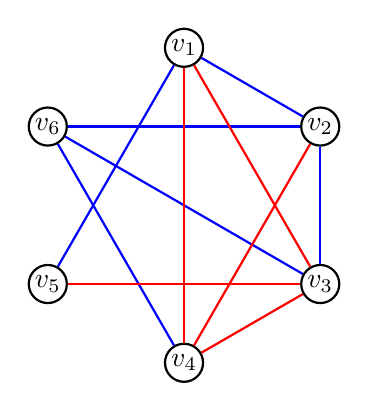
\begin{tikzpicture}
			\tikzset{punkt/.style={circle, thick, draw=black, minimum width=0.2cm,inner sep=1}}
			\node[punkt] at (0.0, 2.0) (a) {$v_1$};
			\node[punkt] at (1.73, 1.0) (b) {$v_2$};
			\node[punkt] at (1.73, -1.0) (c) {$v_3$};
			\node[punkt] at (0.0, -2.0) (d) {$v_4$};
			\node[punkt] at (-1.73, -1.0) (e) {$v_5$};
			\node[punkt] at (-1.73, 1.0) (f) {$v_6$};
			%\draw (0,0) circle [radius=2];

			% Blue edges
			\draw [thick, draw=blue] (a) -- (b);
			\draw [thick, draw=blue] (b) -- (c);
			\draw [thick, draw=blue] (e) -- (a);
			\draw [thick, draw=blue] (f) -- (d);
			\draw [thick, draw=blue] (f) -- (b);
			\draw [thick, draw=blue] (f) -- (c);

			% Red edges
			\draw [thick, draw=red] (a) -- (c);
			\draw [thick, draw=red] (c) -- (d);
			\draw [thick, draw=red] (b) -- (d);
			\draw [thick, draw=red] (c) -- (e);
			\draw [thick, draw=red] (a) -- (d);
		\end{tikzpicture}
		\caption{A graph $G$ with a $2$-edge coloring}
		\label{fig:cliques_and_neighbours}
	\end{figure}
	We see that $\mathcal{C}(G; 3) = \left\{G|_{\{v_1, v_2, v_3\}}, G|_{\{v_2, v_3, v_{6}\}}\right\}$ additionally we see that $\mathcal{N}(v_3; red) = \left\{v_1, v_{4}, v_5\right\}$ and $\mathcal{N}(v_3; blue) = \left\{v_2, v_{6}\right\}$.
\end{example}

\section{Existence of Ramsey Numbers}
This section is based upon \cite{rt}[Section 1.1].
\begin{definition}
	Let $\ell_1, \ell_2, \ldots, \ell_r, n \in \mathbb{N}^{+}$ we will write $n \to (\ell_1, \ell_2, \ldots, \ell_{r})$ if for every $r$-edge coloring $\chi: E(K_{n}) \to \left\{c_1, c_2, \ldots, c_{r}\right\}$ on $K_n$, there exists an $i \in \left\{1, 2, \ldots, r\right\}$ such that $\chi$ admits a $c_{i}$-monochromatic clique of order $\ell_{i}$.
\end{definition}
\begin{remark}
	Clearly $\ell_i \geq \ell_i'$ and $n \to (\ell_1, \ell_2, \ldots, \ell_{r})$ implies that $n \to (\ell_1', \ell_2', \ldots, \ell_{r}')$, since given an $r$-edge coloring $\chi: E(K_{n}) \to \left\{c_1, c_2, \ldots, c_{r}\right\}$ on $K_{n}$ there exists an $i \in [r]$ such that $K_n$ has a $c_{r}$-monochromatic clique of order $\ell_{i} \geq \ell_{i}'$.
\end{remark}

\begin{theorem}[Ramsey's Theorem]\label{thm:ramsey_two_colors}
	Let $\ell_1, \ell_2 \geq 2$, then there exists a $n \in \mathbb{N}^{+}$ such that $n \to (\ell_1, \ell_2)$.
\end{theorem}
\begin{proof}
	Clearly $\ell_1 \to (\ell_1, 2)$ and $\ell_2 \to (2, \ell_2)$ (after all either $K_{\ell_{i}}$ is monochromatic or there exist a monochromatic clique of order $2$). We will proceed using induction on $\ell_1 + \ell_{2}$, hence we may assume that $\ell_1 + \ell_2 \geq 6$, with $\ell_1, \ell_2 \geq 3$.
	Additionally by our induction hypothesis we may assume the existence of non-zero $n_1, n_2 \in \mathbb{N}$ such that $n_1 \to (\ell_1, \ell_2 - 1)$ and $n_2 \to (\ell_1 - 1, \ell_2)$. Next let $n := n_1 + n_2$ we will show that $n \to (\ell_1, \ell_2)$. Fix an arbitrary $2$-edge coloring $\chi: E(K_{n}) \to \left\{red, blue\right\}$ on $K_n$ and let $v$ be a vertex in $K_n$, then $v$ is adjacent to $n - 1$ other vertices in $K_{n}$, hence:
	\begin{equation*}
		n_1 + n_2 - 1 = n - 1 = \abs{\mathcal{N}_{\chi}(v; red)} + \abs{\mathcal{N}_{\chi}(v; blue)}
	\end{equation*}
	meaning either $\abs{N_{\chi}(v; red)} \geq n_2$ or $\abs{N_{\chi}(v; blue)} \geq n_1$, by the Generalized Pigeonhole Principle (Theorem \ref{thm:gpp}). Without loss of generality assume that the second inequality holds, namely $\abs{N_{\chi}(v; blue)} \geq n_1$. By our inductive hypothesis, the complete graph:
	\begin{equation*}
		G = \left(N_{\chi}(v; blue), E(K_{n}) \cap (N_{\chi}(v; blue) \times N_{\chi}(v; blue))\right)
	\end{equation*}
	contains either a $red$-monochromatic clique of order $\ell_{1}$ (in which case we are done) or a $blue$-monochromatic clique of order $\ell_{2} - 1$, in which case we note that $v$ is connected to the vertices in $N_{\chi}(v; 2)$ via edges which $\chi$ colors $blue$, and hence $K_n |_{\mathcal{N}_{\chi}(v, blue) \cup \left\{v\right\}}$ is a $blue$-monochromatic clique of order $\ell_{2}$.
\end{proof}

\begin{corollary}\label{cor:ramsey_for_arbitarily_many_colors}
	Let $\ell_1, \ell_2, \ldots, \ell_r \geq 2$, then there exists a $n \in \mathbb{N}^{+}$ such that $n \to (\ell_1, \ell_2, \ldots, \ell_{r})$.
\end{corollary}

\begin{proof}
	We proceed using induction on $r$, the base case $r = 2$ is proven in Theorem \ref{thm:ramsey_two_colors}.
	Next assume that the theorem holds for $r - 1$. From Theorem \ref{thm:ramsey_two_colors}, it follows that there exists a $\ell \in \mathbb{N}^{+}$ such that $\ell \to (\ell_{r - 1}, \ell_{r})$.
	By our induction hypothesis we may find a $n \in \mathbb{N}^{+}$ for which it holds that:
	\begin{equation*}
		n \to (\ell_1, \ell_2, \ldots, \ell_{r - 2}, \ell)
	\end{equation*}
	Now given any $r$-edge coloring $\chi: E(K_n) \to \left\{c_1, c_2, \ldots, c_{r}\right\}$ on $K_n$ we may obtain a $r - 1$-edge coloring $\chi': E(K_{n}) \to \left\{c_1, c_2, \ldots, c_{r-1}\right\}$ on $K_n$ by defining:
	\begin{equation*}
		\chi'(e) = \begin{cases} \chi(e) & \text{ if } \chi(e) \neq c_{r} \\ c_{r - 1} & \text{ if } \chi(e) = c_{r} \end{cases}
	\end{equation*}
	Hence $\chi'$ must either admit a $c_{i}$-monochromatic clique of order $\ell_i$, for some $i \in \left\{1, 2, \ldots, r - 2\right\}$ (in which case we are done) or a $c_{r - 1}$-monochromatic clique of order $\ell$. If the second case holds let $C$ be this $c_{r-1}$-monochromatic clique of order $\ell$, then $\chi$ colors every edge in $C$ with either $c_{r - 1}$ or $c_{r}$. However $\ell$ was chosen so that $\ell \to (\ell_{r - 1}, \ell_r)$, hence $C$ must contain either a $c_{r - 1}$-monochromatic clique of order $\ell_{r - 1}$ or a $c_{r}$-monochromatic clique of order $\ell_{r}$.
\end{proof}

\begin{definition}
	Let $\ell_1, \ell_2, \ldots, \ell_r \in \mathbb{N}^{+}$ the \textit{Ramsey number} $R(\ell_1, \ell_2, \ldots, \ell_{r})$, is the minimal $n \in \mathbb{N}^{+}$ such that $n \to (\ell_1, \ell_2, \ldots, \ell_{r})$, additionally we let $R(\ell; r)$ denote $R(\ell_1, \ell_2, \ldots, \ell_{r})$, with $\ell_1 = \ell_2 = \cdots = \ell_r = \ell$. The Ramsey numbers of the form $R(\ell; 2)$ are called \textit{digaonal Ramsey numbers}.
\end{definition}
\begin{remark}
	The Ramsey number $R(\ell,k)$ can also be thought of as the minimum order an arbitrary graph $G = (V, E)$ must be, to guarantee the existence of a clique of order $\ell$ or a set of $k$ independent vertices, that is there exists a set $U$ of $k$ verticies such that no two verticies in $U$ are adjacent.
\end{remark}
Generally direct computation of Ramsey numbers are extremely difficult, however there is some exceptions, for instance we have $R(2, \ell) = R(\ell, 2) = \ell$, confer the basis step in the proof of Theorem \ref{thm:ramsey_two_colors}, below we present another example.

\begin{example}\label{exmp:R3_3}
	In this example we will show that $R(3, 3) = 6$, we start by showing that $R(3, 3) \leq 6$. Consider an arbitary $2$-edge coloring $\chi: E(K_{6}) \to \left\{red, blue\right\}$ on $K_6$ and let $v$ be a vertex in $K_6$, then $v$ has $5$ adjacent neighbours, by the generalized pigeonhole principle, Theorem \ref{thm:gpp}, there is a color $c$ (either $red$ or $blue$) such that $\abs{\mathcal{N}_{\chi}(v; c)} \geq 3$.

	Without loss of generality we may assume that $c = red$. Next take pairwise distinct $v_1, v_2, v_3 \in \mathcal{N}_{\chi}(v; red)$, then we must have $\chi(v_{i}, v_{j}) = blue$ for pairwise distinct $i, j \in [3]$, otherwise $K_{6} |_{\left\{v, v_i, v_j\right\}}$ would form a $red$-monochromatic clique of order $3$. However this in turn means that $\chi(v_i, v_j) = blue$ for all pairwise distinct $i, j \in [3]$, hence $K_6 |_{\left\{v_1, v_2, v_3\right\}}$ forms a $blue$-monochromatic clique of order $3$.

	On the other hand it is easy to construct a $2$-edge coloring on $K_5$ which admit no monochromatic subclique of order $3$, one example of such a $2$-edge coloring is illustrated in Figure \ref{fig:K5_counter_example}.
	\begin{figure}[H]
		\centering
		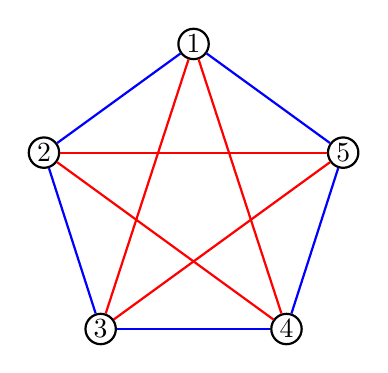
\begin{tikzpicture}
			\tikzset{punkt/.style={circle, thick, draw=black, minimum width=0.2cm,inner sep=1}}
			\node[punkt] at (0.0, 2.0) (a) {$1$};
			\node[punkt] at (-1.9, 0.62) (b) {$2$};
			\node[punkt] at (-1.18, -1.62) (c) {$3$};
			\node[punkt] at (1.18, -1.62) (d) {$4$};
			\node[punkt] at (1.9, 0.62) (e) {$5$};
			%\draw (0,0) circle [radius=2];

			% Blue edges
			\draw [thick, draw=blue] (a) -- (b);
			\draw [thick, draw=blue] (b) -- (c);
			\draw [thick, draw=blue] (c) -- (d);
			\draw [thick, draw=blue] (d) -- (e);
			\draw [thick, draw=blue] (e) -- (a);

			% Red edges
			\draw [thick, draw=red] (a) -- (c);
			\draw [thick, draw=red] (a) -- (d);
			\draw [thick, draw=red] (b) -- (d);
			\draw [thick, draw=red] (b) -- (e);
			\draw [thick, draw=red] (c) -- (e);
		\end{tikzpicture}
		\caption{A 2-edge coloring on $K_{5}$ that admits no monochromatic subclique of order $3$.}
		\label{fig:K5_counter_example}
	\end{figure}
	Finally since $R(3, 3) > 5$ and $R(3, 3) \leq 6$, we obtain that $R(3, 3) = 6$.
\end{example}
\newpage

We might also be interested in when an $r$-edge coloring of a complete graph admits some special monochromatic subgraphs, following this spirit we introduce the following definition:
\begin{definition}
	Let $G_1, G_2, \ldots, G_r$ be graphs, the \textit{generalized Ramsey number} $R(G_1, G_2, \ldots, G_{r})$ is the smallest integer $N$ such that for any $r$-edge coloring $\chi: E(K_N) \to \{c_1, c_2, \ldots, c_{r}\}$ there exists some index $i \in [1; r]$ such that there exists a $c_i$ monochromatic subgraph of $K_n$ which is isomorphic to $G_{i}$.
\end{definition}

It is worth noting that the generalized Ramsey number $R(G_1, G_2, \ldots, G_{r})$ is well defined. This can be seen as follows: let $\ell_j = \abs{V(G_{j})}$ consider the arbitrary $r$-coloring $\chi: E(K_n) \to \{c_1, c_2, \ldots, c_{r}\}$ of $K_n$ with $n = R(\ell_1, \ell_2, \ldots, \ell_{r})$. Then by the definition of $R(\ell_1, \ell_2, \ldots, \ell_{r})$ there exists an $i \in [1; r]$ such that $\chi$ admits a $c_i$-monochromatic clique of order $\ell_i$. The rest follows by the well ordering principle and the fact that $G_i$ is isomorphic to a subgraph of the previously mentioned $c_{i}$-monochromatic clique.

\section{Upper Bounds}\label{sec:upper_bound}
In this section we will prove several upper bounds for both regular and generalized Ramsey numbers, we will start by proving the following upper bound for $R(G_1, G_2, \ldots, G_{r})$.
\begin{theorem}\label{thm:ramsey_upper_bound}
	Let $G_1, G_2, \ldots, G_r$ be graphs with at least $2$ vertices, then:
	\begin{equation*}
		R(G_{1}, G_2, \ldots, G_{r}) \leq 2 - r + \sum_{i = 1}^r R(G_1, \ldots, G_{i - 1}, G_{i}', G_{i + 1}, \ldots, G_{r})
	\end{equation*}
	where the graph $G'$ is obtained from $G$ by deleting one vertex and all of the edges incident to it.
\end{theorem}
\begin{proof}
	For the sake of convenience we will let $R_i = R(G_1, \ldots, G_{i - 1}, G'_{i}, G_{i + 1}, \ldots, G_{r})$ throughout the proof.
	Let $N := 2 - r + \sum_{i = 1}^r R_{i}$ and $\chi$ be an $r$-edge coloring of $K_N$.
	Let $v \in V(K_{N})$, then $v$ is adjacent with $N - 1 = 1 +\sum_{i = 1}^r \left(R_{i} - 1\right)$ other vertices in $K_N$.
	By the Generalized Pigeon Hole Principle (Theorem \ref{thm:gpp}) there exists an $i \in [1; r]$ such that $\abs{\mathcal{N}_{\chi}(v, c_i)} \geq R_{i}$.
	By the definition of $R_i$, we have two cases:
	\begin{enumerate}
		\item Either $\chi$ admits a $c_j$-monochromatic subgraph which is isomorphic with $G_j$, with vertices belonging to $\mathcal{N}_{\chi}(v, c_{i})$, with $j \neq i$, in which case we are done.
		\item Or $\chi$ admits a $c_i$-monochromatic subgraph which is isomorphic with $G'_{i}$ with vertices belonging to $\mathcal{N}_{\chi}(v, c_i)$, of order $\ell_i - 1$, in which case adding $v$ along with the appropriate edges in the set $\left\{\{v, u\} \middle| u \in \mathcal{N}_{\chi}(v, c_{i})\right\}$ forms a $c_i$-monochromatic subgraph which is isomorphic with $G_{i}$. \qedhere
	\end{enumerate}
\end{proof}

In particular Theorem \ref{thm:ramsey_upper_bound}, with $G_i = K_{\ell_{i}}$ implies that:
\begin{equation}\label{eq:cor_1}
	R \left(\ell_1, \ell_2, \ldots, \ell_{r}\right) \leq 2 - r +  \sum_{i = 1}^r R(\ell_1, \ldots, \ell_{i - 1}, \ell_i, \ell_{i + 1}, \ldots, \ell_{r})
\end{equation}

\newpage
\begin{corollary}\label{cor:R3r}
	Let $r \in \mathbb{N}^{+}$ then $R(3; r) \leq 3r!$.
\end{corollary}
\begin{proof}
	We will prove the corollary using induction on $r$. Clearly the result holds in the case where $r = 1$. Next for an arbitrary $r \in \mathbb{N}^{+}$ it follows by Equation \eqref{eq:cor_1}, that:
	\begin{equation}\label{eq:R3r}
		R(3; r) \stackrel{(a)}{\leq} r R(2, 3, \ldots, 3) \stackrel{(b)}{=} r R(3; r - 1) \stackrel{(c)}{=} 3r (r - 1)! = 3r!
	\end{equation}
	where $(a)$ follows by Equation \eqref{eq:R3r}, $(b)$ follows since letting $n := R(2, 3, \ldots, 3)$ we see that every $r$-edge coloring on $K_n$ either admits a monochromatic clique of order $2$ of the appropriate color or we actually have $(r - 1)$-edge coloring on $K_n$. Finally $(c)$ follows directly by the induction hypothesis.
\end{proof}


%\begin{proposition}\label{prop:upper_bounds_form_ramseys_theorem}
%	Let $G, H$ be graphs with $\abs{V(G)}, \abs{V(H)} \geq 2$ and let $G'$ and $H'$ be subgraphs of $G$ and $H$ respectively obtained by deleting a vertex and the appropriate edges, then:
%	\begin{equation*}
%		R(G, H) \leq R(G', H) + R(G, H')
%	\end{equation*}
%\end{proposition}
%We will omit the proof, but note that the basic argument is the same as in the proof of Theorem \ref{thm:ramsey_two_colors}.
The following Corollary is a natural consequence of Theorem \ref{thm:ramsey_upper_bound} and the fact that $R(\ell, 2) = R(2, \ell) = \ell$ for all $\ell \geq 2$.
\begin{corollary}
	Let $\ell, k \in \mathbb{N}$ with $\ell, k \geq 2$, then $R(\ell, k) \leq \binom{\ell + k - 2}{\ell - 1}$
\end{corollary}
\begin{proof}
	We will apply induction on $\ell + k$, in the case where $\ell = 2$ we get that
	\begin{equation*}
		R(\ell, k) = k = \frac{k!}{(k - 1)!} = \binom{k + \ell - 2}{\ell - 1}
	\end{equation*}
	The case where $k = 2$ follows in a similar manner. Next we assume that $\ell, k \geq 3$, then:
	\begin{align*}
		R(\ell, k) \stackrel{(a)}{\leq} R(\ell - 1, k) + R(\ell, k - 1) & \stackrel{(b)}{\leq} \binom{(\ell - 1) + k - 2}{(\ell - 1) - 1} + \binom{\ell + (k - 1) - 2}{\ell - 1} \\
		                                                                & =  \frac{(\ell + k - 3)!}{(\ell - 2)!(k - 1)!} + \frac{(\ell + k - 3)!}{(\ell - 1)!(k - 2)!}           \\
		                                                                & =  \frac{(\ell + k - 3)!((\ell - 1) + (k - 1))}{(\ell - 1)!(k - 1)!}
		= \binom{\ell + k - 2}{\ell - 1}
	\end{align*}
	Where $(a)$ follows by Equation \eqref{eq:cor_1} and $(b)$ directly from the induction hypothesis.
\end{proof}

\begin{corollary}\label{cor:upper_bounds_from_ramseys_theorem_even}
	Let $G, H$ be graphs with at least two edges and let $G'$ and $H'$ be subgraphs of $G$ and $H$ respectively obtained by deleting a vertex and the appropriate edges, then if both $R(G', H)$ and $R(G, H')$ are even, then:
	\begin{equation*}
		R(G, H) \leq R(G', H) + R(G, H') - 1
	\end{equation*}
\end{corollary}
\begin{proof}
	Assume for the sake of contradiction that the inequality does not hold, then by Theorem \ref{thm:ramsey_upper_bound}, we must have $N := R(G, H) = R(G', H) + R(G, H')$ and hence there exists an $2$-edge coloring $\chi: E(K_{N - 1}) \to \left\{red, blue\right\}$ of $K_{N - 1}$ which admits no $red$-monochromatic subgraphs which are isomorphic to $G$ and no $blue$-monochromatic subgraph which are isomorphic to $H$. For all $v \in V(K_{N - 1})$ we thus must have:
	\begin{equation*}
		\abs{\mathcal{N}_{\chi}(v; red)} \leq R(G', H) - 1 \text{ and } \abs{\mathcal{N}_{\chi}(v; blue)} \leq R(G, H') - 1
	\end{equation*}
	since we would otherwise have a $red$(or $blue$)-monochromatic subgraph which is isomorphic to $G$ (or $H$). Next since $v$ is adjacent to $N - 2 = R(G', H) + R(G, H') - 2$ vertices we see that we must have:
	\begin{equation*}
		\abs{\mathcal{N}_{\chi}(v; red)} = R(G', H) - 1 \text{ and } \abs{\mathcal{N}_{\chi}(v; blue)} = R(G, H') - 1
	\end{equation*}
	Next let $k := \abs{\left\{e \in E(K_{N - 1}) | \chi(e) = red\right\}}$ that is $k$ is the number of edges which $\chi$, colors $red$. Thus we may also compute $k$ as:
	\begin{equation}\label{eq:k_is_not_integer}
		k = \frac{1}{2}\sum_{u \in V(K_{N - 1})}\abs{\mathcal{N}_{\chi}(u; red)} = \frac{1}{2}(N - 1)(R(G', H) - 1)
	\end{equation}
	however both $N-1$ and $R(G', H) - 1$ are odd by our assumptions, combining this with Equation \eqref{eq:k_is_not_integer}, implies that $k$ is not natural number a clear contradiction.
\end{proof}

\section{Lower Bounds and the Probabilistic Method}\label{sec:lower_bound}
The probabilistic methodprobability was pioneered by Paul Erdős, and it is generally used throughout combinatorics to establish various lower bounds using methods from probability theory, for graph Ramsey theory it yields some of the best lowerbounds for large Ramsey numbers. Suppose we wish to find a lower bound for $R(\ell_1, \ell_2, \ldots,  \ell_{r})$ the basic idea, at least when applying the method to graph Ramsey theory is to consider a random $r$-edge coloring $\chi$ on a the complete graph $K_{N}$. If the probability, that there exists no indices $i \in [1; r]$ such that $\chi$ admits a $c_{i}$-monochromatic clique of order $\ell_{i}$, is less than $1$, then we must have:
\begin{equation*}
	R(\ell_1, \ell_2, \ldots, \ell_{r}) > N
\end{equation*}
We will need the following lemma, which we state without proof.

\begin{lemma}[Stirlings formula]\label{lem:stirling}
	Let $n \in \mathbb{N}$, then:
	\begin{equation*}
		n! > \sqrt{2 \pi n} \left(\frac{n}{\e}\right)^{n}
	\end{equation*}
\end{lemma}
We now state and prove the main theorem of this section.
\begin{theorem}
	Let $r, \ell \geq 2$, then:
	\begin{equation*}
		R(\ell; r) > \frac{\left(2\pi \ell\right)^{\frac{1}{2\ell}}\ell \sqrt{r}^{\ell}}{r^{\frac{1}{2\ell}}\e}
	\end{equation*}
\end{theorem}
\begin{proof}
	Let $N \geq \ell$ be arbitrary for now. Let $\chi: E(K_N) \to \left\{c_1, c_2, \ldots, c_{r}\right\}$ be a random $r$-edge coloring, with each edge $e$ colored uniformly and independently of the other edges, that is $\mathbb{P}(\chi(e) = c_{i}) = \frac{1}{r}$ for every $i \in [1; r]$. Enumerate the $\ell$-cliques of $K_{N}$ as $C_1, C_2, \ldots, C_{\binom{N}{\ell}}$ and consider the stochastic variables $X_1, X_2, \ldots X_{\binom{N}{\ell}}$ as:
	\begin{equation*}
		X_i = \begin{cases}
			1 & \text{ if } \abs{\chi(E(G \vert_{C_i}))} = 1 \\
			0 & \text{ otherwise }
		\end{cases}
	\end{equation*}
	that is $X_i$ is an indicator function which indicates if the clique $C_i$ is monochromatic under $\chi$. Next notice that
	\begin{equation}\label{eq:prop_mon_clique}
		\mathbb{P}(X_i = 1) = r \cdot \left(\frac{1}{r}\right)^{\binom{\ell}{2}} = r \cdot \left(\frac{\sqrt{r}}{\sqrt{r}^{\ell}}\right)^\ell
	\end{equation}
	since $\abs{E(G \vert_{C_i})} = \binom{\ell}{2} = \frac{\ell^2 - \ell}{2}$. Thus:
	\begin{equation}\label{eq:prob_method}
		\mathbb{E} \left[\sum_{i = 1}^{\binom{N}{\ell}} X_{i}\right]
		= \sum_{i = 1}^{\binom{N}{\ell}} \mathbb{P}(X_i = 1)
		\stackrel{(a)}{\leq} \frac{N^{\ell}}{\ell!} \frac{r}{r^{\binom{\ell}{2}}}
		\stackrel{(b)}{<} \frac{N^{\ell}r}{\sqrt{2\pi \ell} \left(\frac{\ell}{\e}\right)^{\ell}}   \left(\frac{\sqrt{r}}{\sqrt{r}^{\ell}}\right)^{\ell}
		= \frac{r}{\sqrt{2\pi\ell}} \left(\frac{N \e \sqrt{r}}{\ell \sqrt{r}^{\ell}}\right)^{\ell}
	\end{equation}
	where $(a)$ follows by Equation \eqref{eq:prop_mon_clique} and $\frac{N!}{(N - \ell)!} = \prod^N_{k = N - \ell + 1} k < N^{\ell}$ and $(b)$ by Stirlings formula (Lemma \ref{lem:stirling}). \\
	The rest follows as $\frac{r}{\sqrt{2\pi\ell}} \left(\frac{N \e \sqrt{r}}{\ell \sqrt{r}^{\ell}}\right)^{\ell} \geq 1$ if and only if $N \geq \frac{\ell \sqrt{r}^{\ell}}{\e \sqrt{r}} \left(\frac{\sqrt{2\pi\ell}}{r}\right)^{\frac{1}{\ell}}$. Thus since inequality $(b)$ is strict we see that $R(\ell; r) > \frac{\ell \sqrt{r}^{\ell}}{\e \sqrt{r}} \left(\frac{\sqrt{2\pi\ell}}{r}\right)^{\frac{1}{\ell}}$.
	%Now if $\frac{r}{\sqrt{2\pi\ell}} \leq 1$, then setting $N := \frac{\ell\sqrt{r}^{\ell}}{e \sqrt{r}}$ implies $\mathbb{E} \left[\sum_{i = 1}^{\binom{N}{\ell}} X_{i}\right] < 1$, by Equation \eqref{eq:prob_method}, meaning $R(\ell; r) > N$. Alternately if $\frac{r}{\sqrt{2\pi\ell}}$ setting $N := \frac{\ell \sqrt{r}^{\ell}}{\e \sqrt{r}} \left(\frac{\sqrt{2\pi\ell}}{r}\right)^{\frac{1}{\ell}}$, then Equation \eqref{eq:prob_method}, once again gives $\mathbb{E} \left[\sum_{i = 1}^{\binom{N}{\ell}} X_{i}\right] < 1$ concluding the proof.
\end{proof}
%\begin{theorem}
%	Let $\ell \geq 3$ then $R(\ell, \ell) > \frac{\ell}{\e \sqrt{2}} 2^{\ell / 2}$.
%\end{theorem}
%\begin{proof}
%	Let $\chi: E(K_N) \to \left\{red, blue\right\}$ be a random $2$-edge coloring with, we will assume the $\chi(e)$ of is chosen uniformly and independently. Let $C$ be a subgraph of $K_N$ such that $C$ forms a clique and $A_C$ be the event that $\abs{\chi(E(G \vert_{C}))} = 1$, meaning $C$ is monochromatic. Then:
%	\begin{equation*}
%		\mathbb{P}(A_C) = 2 \left(\frac{1}{2} \right)^{\binom{\ell}{2}} = 2^{1 - \binom{\ell}{2}}
%	\end{equation*}
%	since all $\binom{\ell}{2}$ edges of $C$ is must be colored the same color by $\chi$. Let $\mathcal{C}(K_N;\ell)$ be the set of cliques of $K_N$ of order $\ell$, then:
%	\begin{equation*}
%		\mathbb{P} \left(\bigcup_{C \in \mathcal{C}(K_{N}; \ell)} A_{C}\right) \leq \sum_{C \in \mathcal{C}(K_N; \ell)} \mathbb{P}(A_{C}) = \binom{N}{\ell} 2^{1 - \binom{\ell}{2}}
%	\end{equation*}
%	which follows as $\mathcal{C}(K_N; \ell) = \binom{N}{\ell}$. Now if this probability is strictly less than $1$, we must have:
%	\begin{equation*}
%		\mathbb{P}\left(\bigcap_{C \in \mathcal{C}(K_N; \ell)} \overline{A_{C}}\right) = 1 - \mathbb{P} \left(\bigcup_{C \in \mathcal{C}(K_{N}; \ell)} A_{C}\right) \neq 0
%	\end{equation*}
%	where $\overline{A_C}$ is the complement of $A_C$, meaning it is the event that $C$ is not a monochromatic clique. Meaning if this is the case then there must exist a $2$-edge coloring which emits no monochromatic clique of order $\ell$. However it remains to find an integer $N$ such that $\mathbb{P} \left(\bigcup_{C \in \mathcal{C}(K_{N}; \ell)} A_{C}\right) < 1$. We start by computing an upper bound, for the probability that there is at least one monochromatic clique in $K_N$:
%	\begin{equation*}
%		\mathbb{P} \left(\bigcup_{C \in \mathcal{C}(K_{N}; \ell)} A_{C}\right) \leq \binom{N}{\ell} 2^{1 - \binom{\ell}{2}} \stackrel{(a)}{\leq} \frac{N^{\ell}}{\ell!} 2^{1 - \binom{\ell}{2}} \stackrel{(b)}{<} \frac{2}{\sqrt{2\pi \ell}} \left(\frac{\e \sqrt{2} N}{\ell 2^{\ell/2}}\right)^{\ell}
%	\end{equation*}
%	where inequality $(a)$ follow as $\binom{N}{\ell} = \frac{N(N - 1)\cdots(N - \ell + 1)}{\ell!} \leq \frac{N^{\ell}}{\ell!}$ and $(b)$ by Stirlings formula (Lemma \ref{lem:stirling}) and the fact that:
%	\begin{equation*}
%		2^{1 - \binom{\ell}{2}} = 2 \cdot 2^{(-\ell^2 + \ell) / 2} = \frac{2 \cdot \sqrt{2}^{\ell}}{2^{\frac{\ell^2}{2}}}
%	\end{equation*}
%	The rest follows by setting $N = \frac{\ell}{\e \sqrt{2}} 2^{\ell / 2}$.
%\end{proof}

The following theorem are based upon \cite{fg_and_rt}[Theorem 5.5] and gives us our first lower bound for the non-diagonal Ramsey numbers, note that the theorem can also be applied recursively to give a lower bound a general Ramsey number $R(\ell_1, \ell_2, \ldots, \ell_{r})$, via a process similar to the approach used in the proof of Corollary \ref{cor:ramsey_for_arbitarily_many_colors}.
\begin{theorem}
	Let $\ell \geq 2$, there exists a $c_{\ell} > 0$ such that:
	\begin{equation*}
		R(\ell, k) \geq c_{\ell} \left(\frac{k}{\log(k)}\right)^{\frac{\ell - 1}{2}}
	\end{equation*}
	for all $k \geq 2$.
\end{theorem}
We will only give a sketch of the proof.
\begin{proof}[Proof (Sketch)]
	Let $N = \floor{c_{\ell} \left(\frac{k}{\log(k)}\right)^{\frac{\ell - 1}{2}}}$\footnote{Please note that $N$, is not actually fixed, but rahter $N$ depends on $c_{\ell}$.} and $\chi: E(K_N) \to \left\{red, blue\right\}$ be a random $2$-edge coloring on $K_N$, with each edge $e \in E(K_{N})$ colored independently of the others, and with $\mathbb{P}(\chi(e) = red) = \frac{1}{N^{\frac{2}{\ell  - 1}}}$. Next enumerate the $\ell$ and $k$ cliques of $K_N$ as $C_1, C_2, \ldots, C_{\binom{N}{\ell}}$ and $C'_1, C'_2, \ldots, C'_{\binom{N}{k}}$ respectively. We will define the stochastic variables $X_1, X_2, \ldots, X_{\binom{N}{\ell}}$ and $Y_1, Y_2, \ldots, Y_{\binom{N}{k}}$ as:
	\begin{equation*}
		X_i = \begin{cases}
			1 & \text{ if } \chi(E(G \vert_{C_i})) = \left\{red\right\} \\
			0 & \text{ otherwise }
		\end{cases}
	\end{equation*}
	and
	\begin{equation*}
		Y_i = \begin{cases}
			1 & \text{ if } \chi(E(G \vert_{C'_i})) = \left\{blue\right\} \\
			0 & \text{ otherwise }
		\end{cases}
	\end{equation*}
	Letting $p := \mathbb{P}(\chi(e) = red)$ we see that:
	\begin{equation*}
		\mathbb{E} \left[\sum_{i = 1}^{\binom{N}{\ell}} X_i + \sum_{i = 1}^{\binom{N}{k}} Y_{i}\right] \stackrel{a}{=} \binom{N}{\ell} p^{\binom{\ell}{2}} + \binom{N}{k}(1 - p)^{\binom{k}{2}}
	\end{equation*}
	where $(a)$ follows since each edge is colored independently meaning $\mathbb{P} \left(X_i = 1\right) = p^{\binom{\ell}{2}}$ since each of the $\binom{\ell}{2}$ edges in $G \vert_{C_i}$ must be colored $red$ by $\chi$ and similarly $Y_j = 1$ if and only if each edge in $G \vert_{C'_{i}}$ is colored $blue$ by $\chi$. Finally we note that if $c_{\ell}$ is chosen sufficiently small, then $\binom{N}{\ell} p^{\binom{\ell}{2}} + \binom{N}{k}(1 - p)^{\binom{k}{2}} < 1$.
\end{proof}

\section{Exact Values of Small Ramsey Numbers}\label{sec:exact_values}
In this section we compute the exact values of some of the smaller ramsey numbers, using some of the upper bounds which we proved in Section \ref{sec:upper_bound}. The section will be based upon \cite{emogrt}[Chapter 2].
\begin{theorem}\label{thm:small_ramsey_numbers}
	$R(3, 4) = 9, R(3, 5) = 14$ and $R(4, 4) = 18$.
\end{theorem}
\begin{proof}
	by Corollary \ref{cor:upper_bounds_from_ramseys_theorem_even}, we have:
	\begin{equation}\label{eq:R3_4}
		R(3, 4) \leq R(2, 4) + R(3, 3) - 1 = 9
	\end{equation}
	since $R(2, 4) = 4$ and $R(3, 3) = 6$ by Example \ref{exmp:R3_3}. More over by Theorem \ref{thm:ramsey_upper_bound} and Equation \eqref{eq:R3_4} we have:
	\begin{equation}\label{eq:R3_5}
		R(3, 5) \leq R(2, 5) + R(3, 4) \leq 5 + 9 = 14
	\end{equation}
	If we can construct a $2$-edge coloring $\chi: E(K^{*}_{13}) \to \left\{red, blue\right\}$ on $K^{*}_{13}$ with no $red$-clique of order $3$ and no $blue$ clique of order $5$, then we may conclude that $R(3, 5) = 14$ and hence $R(3, 4) = 9$ by Equations \eqref{eq:R3_4} and \eqref{eq:R3_5}. It is in fact the case that we may construct such a $2$-edge coloring $\chi$ on $K^{*}_{13}$ one example of such a coloring is:
	\begin{equation*}
		\chi(\{i, j\}) = \begin{cases}
			red  & \text{ if } [i - j]_{13} \in \left\{1, 5, 8, 12\right\} \\
			blue & \text{ otherwise }
		\end{cases}
	\end{equation*}
	Please note that $\chi$ is well defined since $-1 \equiv 12 \mod 13$ and $-5 \equiv 8 \mod 13$ and hence $[i - j]_{13} \in \left\{1, 5, 8, 12\right\}$ if and only if $[j - i]_{13} \in \left\{1, 5, 8, 12\right\}$. The fact that $\chi$ admits no $red$-monochromatic cliques of order $3$ and no $blue$-monochromatic cliques of order $5$ is checked via the code in Appendix \ref{app:ramsey_code}.
	Additionally since $R(3, 4) = 14$ we have $R(4, 4) \leq R(3, 4) + R(4, 3) = 18$, once again by Theorem \ref{thm:ramsey_upper_bound}, using this inequality we can show that $R(4, 4) = 18$ by constructing a $2$-edge coloring $\gamma: E(K^{*}_{17}) \to \left\{red, blue\right\}$ which admits no $red$ or $blue$ monochromatic cliques of order $4$. One such $2$-edge coloring is given below:
	\begin{equation*}
		\gamma(\left\{i, j\right\}) = \begin{cases}
			red  & \text{ if } [i -  j]_{17} \in \left\{1, 2, 4, 8, 9, 13, 15, 16\right\} \\
			blue & otherwise
		\end{cases}
	\end{equation*}
	again please note that $\gamma$ is well defined, just like $\chi$, by an identical argument. Again the fact that $\gamma$ admits no $red$ or $blue$ monochromatic cliques of order $5$ is checked via the code in Appendix \ref{app:ramsey_code}.
\end{proof}

For the sake of illustration $K^{*}_{13}$ equiped with the $2$-edge coloring $\chi$ and $K^{*}_{17}$ equiped with the $2$-edge coloring $\gamma$, both from the proof of Theorem \ref{thm:small_ramsey_numbers} is illustated below in Figures \ref{fig:small_ramsey_graphs}
\begin{figure}[H]
	\begin{subfigure}[c]{0.4\textwidth}
		\centering
		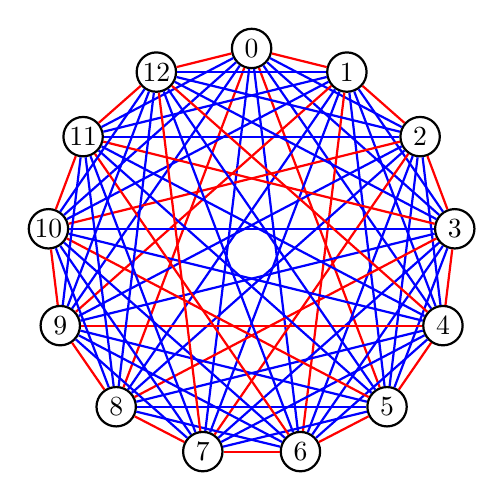
\begin{tikzpicture}
			\tikzset{punkt/.style={circle, thick, draw=black, minimum width=0.5cm,inner sep=0.2}}

			\node[punkt] at (0.0, 2.6) (a) {$0$};
			\node[punkt] at (1.21, 2.3) (b) {$1$};
			\node[punkt] at (2.14, 1.48) (c) {$2$};
			\node[punkt] at (2.58, 0.31) (d) {$3$};
			\node[punkt] at (2.43, -0.92) (e) {$4$};
			\node[punkt] at (1.72, -1.95) (f) {$5$};
			\node[punkt] at (0.62, -2.52) (g) {$6$};
			\node[punkt] at (-0.62, -2.52) (h) {$7$};
			\node[punkt] at (-1.72, -1.95) (i) {$8$};
			\node[punkt] at (-2.43, -0.92) (j) {$9$};
			\node[punkt] at (-2.58, 0.31) (k) {$10$};
			\node[punkt] at (-2.14, 1.48) (l) {$11$};
			\node[punkt] at (-1.21, 2.3) (m) {$12$};
			\draw [thick, draw=red] (a) -- (b);
			\draw [thick, draw=blue] (a) -- (c);
			\draw [thick, draw=blue] (a) -- (d);
			\draw [thick, draw=blue] (a) -- (e);
			\draw [thick, draw=red] (a) -- (f);
			\draw [thick, draw=blue] (a) -- (g);
			\draw [thick, draw=blue] (a) -- (h);
			\draw [thick, draw=red] (a) -- (i);
			\draw [thick, draw=blue] (a) -- (j);
			\draw [thick, draw=blue] (a) -- (k);
			\draw [thick, draw=blue] (a) -- (l);
			\draw [thick, draw=red] (a) -- (m);
			\draw [thick, draw=red] (b) -- (c);
			\draw [thick, draw=blue] (b) -- (d);
			\draw [thick, draw=blue] (b) -- (e);
			\draw [thick, draw=blue] (b) -- (f);
			\draw [thick, draw=red] (b) -- (g);
			\draw [thick, draw=blue] (b) -- (h);
			\draw [thick, draw=blue] (b) -- (i);
			\draw [thick, draw=red] (b) -- (j);
			\draw [thick, draw=blue] (b) -- (k);
			\draw [thick, draw=blue] (b) -- (l);
			\draw [thick, draw=blue] (b) -- (m);
			\draw [thick, draw=red] (c) -- (d);
			\draw [thick, draw=blue] (c) -- (e);
			\draw [thick, draw=blue] (c) -- (f);
			\draw [thick, draw=blue] (c) -- (g);
			\draw [thick, draw=red] (c) -- (h);
			\draw [thick, draw=blue] (c) -- (i);
			\draw [thick, draw=blue] (c) -- (j);
			\draw [thick, draw=red] (c) -- (k);
			\draw [thick, draw=blue] (c) -- (l);
			\draw [thick, draw=blue] (c) -- (m);
			\draw [thick, draw=red] (d) -- (e);
			\draw [thick, draw=blue] (d) -- (f);
			\draw [thick, draw=blue] (d) -- (g);
			\draw [thick, draw=blue] (d) -- (h);
			\draw [thick, draw=red] (d) -- (i);
			\draw [thick, draw=blue] (d) -- (j);
			\draw [thick, draw=blue] (d) -- (k);
			\draw [thick, draw=red] (d) -- (l);
			\draw [thick, draw=blue] (d) -- (m);
			\draw [thick, draw=red] (e) -- (f);
			\draw [thick, draw=blue] (e) -- (g);
			\draw [thick, draw=blue] (e) -- (h);
			\draw [thick, draw=blue] (e) -- (i);
			\draw [thick, draw=red] (e) -- (j);
			\draw [thick, draw=blue] (e) -- (k);
			\draw [thick, draw=blue] (e) -- (l);
			\draw [thick, draw=red] (e) -- (m);
			\draw [thick, draw=red] (f) -- (g);
			\draw [thick, draw=blue] (f) -- (h);
			\draw [thick, draw=blue] (f) -- (i);
			\draw [thick, draw=blue] (f) -- (j);
			\draw [thick, draw=red] (f) -- (k);
			\draw [thick, draw=blue] (f) -- (l);
			\draw [thick, draw=blue] (f) -- (m);
			\draw [thick, draw=red] (g) -- (h);
			\draw [thick, draw=blue] (g) -- (i);
			\draw [thick, draw=blue] (g) -- (j);
			\draw [thick, draw=blue] (g) -- (k);
			\draw [thick, draw=red] (g) -- (l);
			\draw [thick, draw=blue] (g) -- (m);
			\draw [thick, draw=red] (h) -- (i);
			\draw [thick, draw=blue] (h) -- (j);
			\draw [thick, draw=blue] (h) -- (k);
			\draw [thick, draw=blue] (h) -- (l);
			\draw [thick, draw=red] (h) -- (m);
			\draw [thick, draw=red] (i) -- (j);
			\draw [thick, draw=blue] (i) -- (k);
			\draw [thick, draw=blue] (i) -- (l);
			\draw [thick, draw=blue] (i) -- (m);
			\draw [thick, draw=red] (j) -- (k);
			\draw [thick, draw=blue] (j) -- (l);
			\draw [thick, draw=blue] (j) -- (m);
			\draw [thick, draw=red] (k) -- (l);
			\draw [thick, draw=blue] (k) -- (m);
			\draw [thick, draw=red] (l) -- (m);
		\end{tikzpicture}
		\caption{The $2$-edge coloring $\chi$ on $K^{*}_{13}$}
	\end{subfigure}
	\begin{subfigure}[c]{0.6\textwidth}
		\centering
		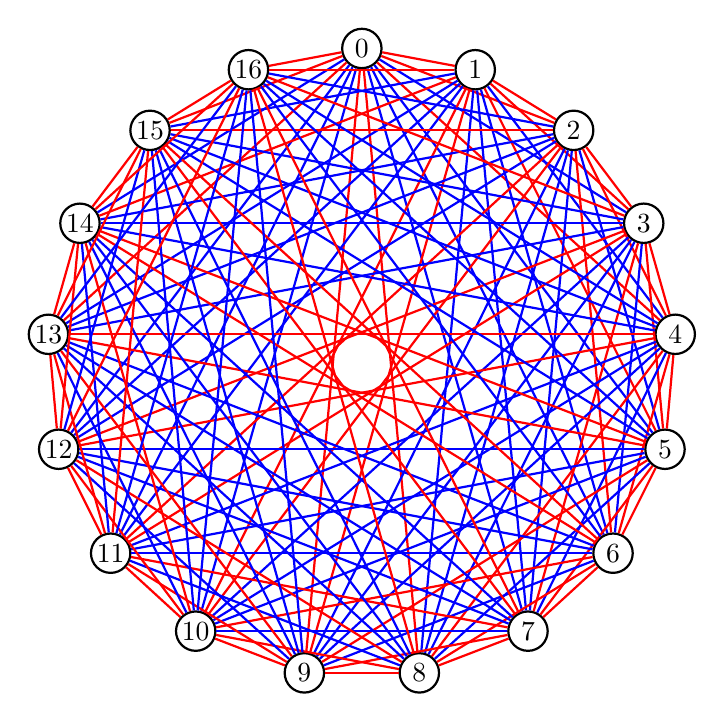
\begin{tikzpicture}
			\tikzset{punkt/.style={circle, thick, draw=black, minimum width=0.5cm,inner sep=0.2}}
			\node[punkt] at (0.0, 4.0) (a) {$0$};
			\node[punkt] at (1.44, 3.73) (b) {$1$};
			\node[punkt] at (2.69, 2.96) (c) {$2$};
			\node[punkt] at (3.58, 1.78) (d) {$3$};
			\node[punkt] at (3.98, 0.37) (e) {$4$};
			\node[punkt] at (3.85, -1.09) (f) {$5$};
			\node[punkt] at (3.19, -2.41) (g) {$6$};
			\node[punkt] at (2.11, -3.4) (h) {$7$};
			\node[punkt] at (0.73, -3.93) (i) {$8$};
			\node[punkt] at (-0.73, -3.93) (j) {$9$};
			\node[punkt] at (-2.11, -3.4) (k) {$10$};
			\node[punkt] at (-3.19, -2.41) (l) {$11$};
			\node[punkt] at (-3.85, -1.09) (m) {$12$};
			\node[punkt] at (-3.98, 0.37) (n) {$13$};
			\node[punkt] at (-3.58, 1.78) (o) {$14$};
			\node[punkt] at (-2.69, 2.96) (p) {$15$};
			\node[punkt] at (-1.44, 3.73) (q) {$16$};
			\draw [thick, draw=red] (a) -- (b);
			\draw [thick, draw=red] (a) -- (c);
			\draw [thick, draw=blue] (a) -- (d);
			\draw [thick, draw=red] (a) -- (e);
			\draw [thick, draw=blue] (a) -- (f);
			\draw [thick, draw=blue] (a) -- (g);
			\draw [thick, draw=blue] (a) -- (h);
			\draw [thick, draw=red] (a) -- (i);
			\draw [thick, draw=red] (a) -- (j);
			\draw [thick, draw=blue] (a) -- (k);
			\draw [thick, draw=blue] (a) -- (l);
			\draw [thick, draw=blue] (a) -- (m);
			\draw [thick, draw=red] (a) -- (n);
			\draw [thick, draw=blue] (a) -- (o);
			\draw [thick, draw=red] (a) -- (p);
			\draw [thick, draw=red] (a) -- (q);
			\draw [thick, draw=red] (b) -- (c);
			\draw [thick, draw=red] (b) -- (d);
			\draw [thick, draw=blue] (b) -- (e);
			\draw [thick, draw=red] (b) -- (f);
			\draw [thick, draw=blue] (b) -- (g);
			\draw [thick, draw=blue] (b) -- (h);
			\draw [thick, draw=blue] (b) -- (i);
			\draw [thick, draw=red] (b) -- (j);
			\draw [thick, draw=red] (b) -- (k);
			\draw [thick, draw=blue] (b) -- (l);
			\draw [thick, draw=blue] (b) -- (m);
			\draw [thick, draw=blue] (b) -- (n);
			\draw [thick, draw=red] (b) -- (o);
			\draw [thick, draw=blue] (b) -- (p);
			\draw [thick, draw=red] (b) -- (q);
			\draw [thick, draw=red] (c) -- (d);
			\draw [thick, draw=red] (c) -- (e);
			\draw [thick, draw=blue] (c) -- (f);
			\draw [thick, draw=red] (c) -- (g);
			\draw [thick, draw=blue] (c) -- (h);
			\draw [thick, draw=blue] (c) -- (i);
			\draw [thick, draw=blue] (c) -- (j);
			\draw [thick, draw=red] (c) -- (k);
			\draw [thick, draw=red] (c) -- (l);
			\draw [thick, draw=blue] (c) -- (m);
			\draw [thick, draw=blue] (c) -- (n);
			\draw [thick, draw=blue] (c) -- (o);
			\draw [thick, draw=red] (c) -- (p);
			\draw [thick, draw=blue] (c) -- (q);
			\draw [thick, draw=red] (d) -- (e);
			\draw [thick, draw=red] (d) -- (f);
			\draw [thick, draw=blue] (d) -- (g);
			\draw [thick, draw=red] (d) -- (h);
			\draw [thick, draw=blue] (d) -- (i);
			\draw [thick, draw=blue] (d) -- (j);
			\draw [thick, draw=blue] (d) -- (k);
			\draw [thick, draw=red] (d) -- (l);
			\draw [thick, draw=red] (d) -- (m);
			\draw [thick, draw=blue] (d) -- (n);
			\draw [thick, draw=blue] (d) -- (o);
			\draw [thick, draw=blue] (d) -- (p);
			\draw [thick, draw=red] (d) -- (q);
			\draw [thick, draw=red] (e) -- (f);
			\draw [thick, draw=red] (e) -- (g);
			\draw [thick, draw=blue] (e) -- (h);
			\draw [thick, draw=red] (e) -- (i);
			\draw [thick, draw=blue] (e) -- (j);
			\draw [thick, draw=blue] (e) -- (k);
			\draw [thick, draw=blue] (e) -- (l);
			\draw [thick, draw=red] (e) -- (m);
			\draw [thick, draw=red] (e) -- (n);
			\draw [thick, draw=blue] (e) -- (o);
			\draw [thick, draw=blue] (e) -- (p);
			\draw [thick, draw=blue] (e) -- (q);
			\draw [thick, draw=red] (f) -- (g);
			\draw [thick, draw=red] (f) -- (h);
			\draw [thick, draw=blue] (f) -- (i);
			\draw [thick, draw=red] (f) -- (j);
			\draw [thick, draw=blue] (f) -- (k);
			\draw [thick, draw=blue] (f) -- (l);
			\draw [thick, draw=blue] (f) -- (m);
			\draw [thick, draw=red] (f) -- (n);
			\draw [thick, draw=red] (f) -- (o);
			\draw [thick, draw=blue] (f) -- (p);
			\draw [thick, draw=blue] (f) -- (q);
			\draw [thick, draw=red] (g) -- (h);
			\draw [thick, draw=red] (g) -- (i);
			\draw [thick, draw=blue] (g) -- (j);
			\draw [thick, draw=red] (g) -- (k);
			\draw [thick, draw=blue] (g) -- (l);
			\draw [thick, draw=blue] (g) -- (m);
			\draw [thick, draw=blue] (g) -- (n);
			\draw [thick, draw=red] (g) -- (o);
			\draw [thick, draw=red] (g) -- (p);
			\draw [thick, draw=blue] (g) -- (q);
			\draw [thick, draw=red] (h) -- (i);
			\draw [thick, draw=red] (h) -- (j);
			\draw [thick, draw=blue] (h) -- (k);
			\draw [thick, draw=red] (h) -- (l);
			\draw [thick, draw=blue] (h) -- (m);
			\draw [thick, draw=blue] (h) -- (n);
			\draw [thick, draw=blue] (h) -- (o);
			\draw [thick, draw=red] (h) -- (p);
			\draw [thick, draw=red] (h) -- (q);
			\draw [thick, draw=red] (i) -- (j);
			\draw [thick, draw=red] (i) -- (k);
			\draw [thick, draw=blue] (i) -- (l);
			\draw [thick, draw=red] (i) -- (m);
			\draw [thick, draw=blue] (i) -- (n);
			\draw [thick, draw=blue] (i) -- (o);
			\draw [thick, draw=blue] (i) -- (p);
			\draw [thick, draw=red] (i) -- (q);
			\draw [thick, draw=red] (j) -- (k);
			\draw [thick, draw=red] (j) -- (l);
			\draw [thick, draw=blue] (j) -- (m);
			\draw [thick, draw=red] (j) -- (n);
			\draw [thick, draw=blue] (j) -- (o);
			\draw [thick, draw=blue] (j) -- (p);
			\draw [thick, draw=blue] (j) -- (q);
			\draw [thick, draw=red] (k) -- (l);
			\draw [thick, draw=red] (k) -- (m);
			\draw [thick, draw=blue] (k) -- (n);
			\draw [thick, draw=red] (k) -- (o);
			\draw [thick, draw=blue] (k) -- (p);
			\draw [thick, draw=blue] (k) -- (q);
			\draw [thick, draw=red] (l) -- (m);
			\draw [thick, draw=red] (l) -- (n);
			\draw [thick, draw=blue] (l) -- (o);
			\draw [thick, draw=red] (l) -- (p);
			\draw [thick, draw=blue] (l) -- (q);
			\draw [thick, draw=red] (m) -- (n);
			\draw [thick, draw=red] (m) -- (o);
			\draw [thick, draw=blue] (m) -- (p);
			\draw [thick, draw=red] (m) -- (q);
			\draw [thick, draw=red] (n) -- (o);
			\draw [thick, draw=red] (n) -- (p);
			\draw [thick, draw=blue] (n) -- (q);
			\draw [thick, draw=red] (o) -- (p);
			\draw [thick, draw=red] (o) -- (q);
			\draw [thick, draw=red] (p) -- (q);
		\end{tikzpicture}
		\caption{The $2$-edge coloring $\gamma$ on $K^{*}_{17}$}
	\end{subfigure}
	\caption{The two 2-edge colorings described in the proof of Theorem \ref{thm:small_ramsey_numbers} illustrated.}
	\label{fig:small_ramsey_graphs}
\end{figure}


Before moving on we will need one additional concept, introduced in the following definition:
\begin{definition}\label{def:set_sum_free}
	Let $(G, +)$ be an abelian group, then the subset $S \subseteq G$ is called \textit{sum-free} if the equation $x + y = z$ has no solution in $S$.
\end{definition}

Some parts of the proof of the following Theorem is inspired by \cite{graph_theory}[Exercise 12.3.4]
\begin{theorem}\label{thm:R3_3_3}
	We have $R(3, 3, 3) = 17$.
\end{theorem}
\begin{proof}
	We start by showing that any $3$-edge coloring $\chi: E(K_{17}) \to \left\{red, blue, green\right\}$ admits a monochromatic clique of order $3$. Let $v \in V(K_{17})$, by the generalized pigeonhole principle (Theorem \ref{thm:gpp}), there exists a color $c \in \left\{red, blue, green\right\}$ such that $\abs{\mathcal{N}_{\chi}(v; c)} \geq 6$. Assume without loss of generalization that $c = red$, then we may assume that $\chi\left(E(K_{17} \vert_{\mathcal{N}_{\chi}(v; c)})\right) = \left\{blue, green\right\}$, otherwise we would have a $red$-monochromatic clique of order $3$. However since $R(3, 3) = 6$, this means that $\chi$ admits either a $blue$ or $green$ monochromatic clique of order $3$.

	Next we will show that $R(3, 3, 3) > 16$, we will do this by constructing a $3$-edge coloring $\gamma$ on the complete graph $K$ with vertex set $\mathbb{Z}_2[X] / \gen{X^4 + X + 1}$\footnote{Which is of course isomorphic to $\mathbb{F}_{16}$, however it will be move convinient for us to work from this polynomial view.}. We will construct $3$ cosets $S_{red}, S_{blue}, S_{green}$ which partition $\mathbb{Z}_2[X] / \gen{X^4 + X + 1}$, and assign a color to the edge $\left\{v, u\right\}$ according to which coset $v + u$ belongs to. To start let:
	\begin{equation*}
		S_{red} := \left\{X^3, X^2 + X^{3}, X + X^{3}, 1 + X + X^2 + X^3 , 1\right\}
	\end{equation*}
	Note that $S_{red}$ is a subgroup of the multiplicative group $(\mathbb{Z}_2[X] / \gen{X^4 + X + 1})^{*}$, additionally we note that $S_{red}$ is sum-free, which is easy albeit cumbersome to check. Similarly we let $A_{blue} := X S_{red}$ and $S_{green} := X^2 S_{red}$, these cosets must also be sum-free since $a + b = c$ with $a, b, c \in S_{blue}$ or $a, b, c \in S_{green}$ would imply:
	\begin{equation*}
		Xa' + Xb' = Xc' \implies a' + b' = c' \text{ with } a', b', c' \in S_{red}
	\end{equation*}
	or
	\begin{equation*}
		X^{2}a' + X^{2}b' = X^{2}c' \implies a' + b' = c' \text{ with } a', b', c' \in S_{red}
	\end{equation*}
	respectively, since $\mathbb{Z}_2[X] / \gen{X^4 + X + 1}$ is a finite field and hence a domain. Define $\gamma(\left\{v, u\right\}) = c$ if and only if $v + u \in S_{c}$, additionally we note that $\gamma$ is well defined as $v \neq u$ and $\Char(\mathbb{Z}_2[X] / \gen{X^4 + X + 1}) = 2$. Assume for the sake of contradiction that $\gamma$ admits a $c$-monochromatic clique of order $3$, that is there exists $u, v, w \in V(K) = \mathbb{Z}_2[X] / \gen{X^4 + X + 1}$ such that $u + v, u + w, v + w \in S_c$, then $u + w = (u + v) + (v + w)$ contradicting the fact that $S_c$ is sum-free.
\end{proof}

Finally we present a summary of the exact values and bounds for small Ramsey numbers, below in Table \ref{tab:small_values}:
\begin{table}[H]
	\centering
	\begin{tabular} {||c|c|c|c|c||}
		\hline
		$\ell_1 \setminus \ell_{2}$ & $2$ & $3$  & $4$                     & $5$                      \\
		\hline
		$2$                         & $2$ & $3$  & $4$                     & $5$                      \\
		\hline
		$3$                         & $3$ & $6$  & $9$                     & $14$                     \\
		\hline
		$4$                         & $4$ & $9$  & $18$                    & $\leq31$, $\mathbf{25}$  \\
		\hline
		$5$                         & $5$ & $14$ & $\leq31$, $\mathbf{25}$ & $\leq62$, \textbf{43-48} \\
		\hline
	\end{tabular}
	\caption{Some exact values and bounds for small Ramsey numbers. The bold entries are exact values or best known bounds, if the exact value is unknown, which we have not covered in this project. The bold values are sourced from \cite{small_values}.}
	\label{tab:small_values}
\end{table}

\section{Asymptotic Behaviour of Certain Ramsey Numbers}\label{sec:ass_ramsey}
In this section we will investigate the asymptotic behaviour of certain Ramsey numbers. Starting with $R(\ell; r)$ as $r \to \infty$ and finishing providing an explicit construction using projective planes, which shows that $R(3, \ell) = \Omega(\ell^{3 / 2})$.
\subsection{Asymptotic Behaviour of $R(\ell; r)$ as $r \to \infty$}\label{sec:ramsey_ass}
In this subsection we will briefly investigate the asymptotic behaviour of $R(\ell; r)$ as $r \to \infty$, with $\ell \geq 3$, our primary reference will be \cite{emogrt}[Subsection 2.3]. We will not consider the case where $\ell = 2$, since $R(2; r) = 2$ for all $r \in \mathbb{N}^{+}$.

\begin{definition}
	Let $f: \mathbb{N} \to \mathbb{R}^{+}$, then $f$ is called \textit{super-multiplicative} if
	\begin{equation*}
		f(n + m) \geq f(m)f(n)
	\end{equation*}
	for all $n,m \in \mathbb{N}^{+}$.
\end{definition}

\begin{lemma}\label{lem:limit_of_super_multiplicative}
	Let $f: \mathbb{N} \to \mathbb{R}^{+}$ be a super-multiplicative function, then the limit of $f(k)^{1 / k}$ as $k \to \infty$ exists an is equal to $\sup_{k \in \mathbb{N}^{+}} f(k)^{1 / k}$. Furthermore if $m \in \mathbb{N}^{+}$ is fixed, then there exists some constant $c_m > 0$ such that:
	\begin{equation*}
		f(n) \geq c_{m} f(m)^{n / m}
	\end{equation*}
	for all $n \geq m$.
\end{lemma}
\begin{proof}
	We clearly have $\limsup_{k \to \infty} f(k)^{1/k} \leq \sup_{k \in \mathbb{N}^{+}} f(k)^{1/k}$, next we will show that $\liminf_{k \to \infty} f(k)^{1 / k} \geq \sup_{k \in \mathbb{N}^{+}} f(k)^{1/k}$, by considering two distinct cases, namely $\sup_{k \in \mathbb{N}^{+}} f(k)^{1/k} < \infty$ and $\sup_{k \in \mathbb{N}^{+}} f(k)^{1/k} = \infty$, separately:
	\begin{enumerate}
		\item If $\sup_{k \in \mathbb{N}^{+}} f(k)^{1/k} < \infty$, then for all $\varepsilon > 0$ there exists an $m \in \mathbb{N}^{+}$ such that:
		      \begin{equation*}
			      f(m)^{1/m} > \sup_{k \in \mathbb{N}^{+}} f(k)^{1/k} - \varepsilon
		      \end{equation*}
		      by the definition of $\sup_{k \in \mathbb{N}^+} f(k)^{1/k}$. Let $n \geq m$, then there exists $q, r \in \mathbb{N}$ with $0 \leq r < m$ such that $n = qm + r$ thus:
		      \begin{equation*}
			      f(n) \geq f(qm) f(r) \geq f(m)^q f(r)
		      \end{equation*}
		      Since $f$ is a super-multiplicative function. We note that $q / n \to 1 / m$ and $f(r)^{1/n} \to 1$ as $n \to \infty$, and hence:
		      \begin{equation*}
			      \liminf_{k \to \infty} f(k)^{1/k} \geq f(m)^{1/m} > \sup_{k \in \mathbb{N}^{+}} f(k)^{1/k} - \varepsilon
		      \end{equation*}
		      However $\varepsilon > 0$ was arbitrary and hence we must have:
		      \begin{equation*}
			      \liminf_{k \to \infty} f(k)^{1/k} \geq \sup_{k \in \mathbb{N}^{+}} f(k)^{1/k}
		      \end{equation*}
		      and thus:
		      \begin{equation*}
			      \sup_{k \in \mathbb{N}^{+}} f(k)^{1/k} \leq \liminf_{k \to \infty} f(k)^{1/k} \leq \limsup_{k \to \infty} f(k)^{1/k} \leq \sup_{k \in \mathbb{N}^{+}} f(k)^{1/k}
		      \end{equation*}
		      since $\liminf_{k \to \infty} x_{n} \leq \limsup_{k \to \infty} x_{n}$ for every real sequence $\left\{x_k\right\}_{k = 1}^{\infty}$. Meaning
		      \begin{equation*}
			      \liminf_{k\to \infty} f(k)^{1/k} = \limsup_{k \to \infty} f(k)^{1/k} = \sup_{k \in \mathbb{N}^+} f(k)^{1/k}
		      \end{equation*}
		\item If $\sup_{k \in \mathbb{N}^{+}} f(k)^{1/k} = \infty$, then for every $M > 0$ there exists some $m \in \mathbb{N}^{+}$ such that $f(m)^{1/m} > M$, by writing $n \geq m$ as $n = qm + r$, again for suitable $q, r \in \mathbb{N}$ and repeating the same argument we get that:
		      \begin{equation*}
			      \liminf_{k \to \infty} f(k)^{1/k} \geq f(m)^{1/m} > M
		      \end{equation*}
		      Meaning $\liminf_{k \to \infty} f(k)^{1/k} = \infty$.
	\end{enumerate}
	Finally we will show that if $m \in \mathbb{N}^{+}$ is fixed, then there exists a constant $c_m > 0$ such that $f(n) \geq c_{m} f(m)^{n / m}$ for all $n \geq m$. Once again we may write $n = qm + r$ for suitable $q, r \in \mathbb{N}$ such that $0 \leq r < m$. Then:
	\begin{equation*}
		f(n) \geq f(qm) f(r) \geq f(m)^q f(r) \stackrel{(a)}{=} f(m)^{(n - r) / m} f(r) = \frac{f(r)}{f(m)^{r / m}} f(m)^{n / m}
	\end{equation*}
	The rest follows by setting $c_m := \min \left\{\frac{f(r)}{f(m)^{r / m}} \middle| 0 \leq r \leq m\right\}$, notice that $c_m \neq 0$, singe $f$ is strictly positive.
\end{proof}

We now reach the main result of this subsection.
\begin{proposition}\label{prop:r_ell_k_is_super_multiplicative}
	Let $\ell \geq 3$, then the function $r \mapsto R(\ell; r) - 1$ is super-multiplicative. In particular $\lim_{r \to \infty} \left(R(\ell; r) - 1\right)^{1/r} = \sup_{r \in \mathbb{N}} (R(\ell; r) - 1)^{1 / r}$ and for every $r \in \mathbb{N}^{+}$ there exists a constant $c_r > 0$ such that $R(\ell; r') \geq c_r R(\ell; r)^{r' / r}$ for all $r' \geq r$.
\end{proposition}

The proof of Proposition \ref{prop:r_ell_k_is_super_multiplicative} will use a technique which is normally refereed to as ``blowing-up'' an $r_1$-edge coloring $\chi$ using another $r_2$-edge coloring $\gamma$, on two complete graphs $K_{1}$ and $K_{2}$ respectively. The process creates an $(r_1 + r_2)$-edge coloring $\psi$ on a complete graph with $\abs{V(K_1)} \cdot \abs{V(K_{2})}$ verticies.
Intuitively the process is the following:
We replace each vertex $u \in V(K_{1})$ with a copy of $K_{2}$, denoted by $K_{2}^{(u)}$, with the edges in $K_2^{(u)}$ colored according to $\gamma$, and color the edges joining the verticies in $K_2^{(v)}$ and $K_2^{(w)}$ the same color as $\left\{v, w\right\}$ under $\chi$.

\begin{proof}[Proof of Proposition \ref{prop:r_ell_k_is_super_multiplicative}]
	Let $r_{1}, r_2 \in \mathbb{N}^{+}$ with $r_1, r_2 \geq 2$, let $n = R(\ell; r_{1}) - 1$ and $m = R(\ell; r_{2}) - 1$. Let $\chi$ and $\gamma$, be a $r_{1}$-edge-coloring or a $r_2$-edge-coloring on the complete graphs $K_V, K_U$ with vertex sets $V := \left\{v_1, v_2, \ldots, v_{n}\right\}$ and $U := \left\{u_1, u_2, \ldots, u_{m}\right\}$ respectively.
	For the sake of simplicity we will without loss of generalization assume that the codomains of $\chi$ and $\gamma$ are disjoint\footnote{If the codomains are intersecting, simply compose either one of $\chi$ and $\gamma$, with a suitable bijection from its codomain to another finite set of colors.}. We will blow-up $\chi$ using $\gamma$ in order to construct a $(r_1 + r_2)$-edge coloring $\psi$ on the complete graph $K_{W}$ with vertex set $W := \left\{w_{i, j} | i \in [1; n], j \in [1; m]\right\}$ clearly $\abs{W} = nm$. We can construct a $(r_1 + r_2)$-edge coloring $\psi$, which admits no monochromatic cliques of order $\ell$, by blowing up $\chi$ with $\gamma$, since $\chi$ and $\gamma$ admits no monochromatic cliques of order $\ell$\footnote{The intuition here is that we have no cliques of order $\ell$, between copies of $K_{U}$ and no cliques contained within each copy of $K_{U}$, due to the properties of $\chi$ and $\gamma$.}.
	That is by defining $\psi$ as:
	\begin{equation*}
		\psi(\left \{w_{i,j}, w_{i', j'}\right\}) := \begin{cases}
			\chi(\left\{v_{i}, v_{i'}\right\})   & \text{ if } j = j' \\
			\gamma(\left\{u_{j}, u_{j'}\right\}) & otherwise          \\
		\end{cases}
	\end{equation*}
	Hence:
	\begin{equation*}
		R(\ell; r_{1} + r_{2}) - 1 \geq mn = (R(\ell; r_{1}) - 1)(R(\ell; r_{2}) - 1)
	\end{equation*}
	The rest follows directly by Lemma \ref{lem:limit_of_super_multiplicative}.
\end{proof}

\begin{corollary}\label{cor:limit_of_R}
	Let $\ell \geq 3$, then $\lim_{r \to \infty} R(\ell; r)^{1/r} = \sup_{r \in \mathbb{N}^{+}} (R(\ell; r) - 1)^{1/r}$
\end{corollary}
\begin{proof}
	We have $\lim_{r \to \infty} \frac{\left(R(\ell; r) - 1\right)^{1/r}}{R(\ell;r)^{1/r}} = \lim_{r \to \infty} \left(1 -  \frac{1}{R(\ell;r)}\right)^{1 / r} = 1$ since $\lim_{r \to \infty} \frac{1}{R(\ell; r)} = 0$, thus $\lim_{r \to \infty} R(\ell; r) ^{1/r} = \lim_{r \to \infty} \left(R(\ell; r) - 1\right)^{1/r} = \sup_{r \in \mathbb{N}^{+}} (R(\ell; r) - 1)^{1/r}$ by Proposition \ref{prop:r_ell_k_is_super_multiplicative}.
\end{proof}

From Corollary \ref{cor:limit_of_R} we see that:
\begin{equation*}
	\lim_{r \to \infty} R(3; r)^{1 / r} \geq \max \left\{(R(3; 2) - 1)^{1 / 2}, (R(3; 3) - 1)^{1/3}\right\}  = \max \left\{5^{1/2}, 16^{1/3}\right\} \geq \frac{5}{2}
\end{equation*}
Since $R(3, 3) = 6$ and $R(3, 3, 3) = 17$, by Example \ref{exmp:R3_3} and Theorem \ref{thm:R3_3_3}. More over we see that $R(3; r) \geq c_r (5 / 2)^r$, for some constant $c_r > 0$ and all $r \geq 2$ by Lemma \ref{lem:limit_of_super_multiplicative}. In subsection \ref{sub:schur_bounds_and_ass}, we will show that $R(3; r)$ grows even more rapidly, by relating it to a different construct.
Finally we note the following conjecture by Paul Erdős:
\begin{conjecture}[Erdős]\label{conj:erdos_limit}
	The limit of $R(3; r)^{1/r}$ as $r \to \infty$ is infinity.
\end{conjecture}
If Conjecture \ref{conj:erdos_limit} holds, then $\ell \geq 3$ implies that $\lim_{r \to \infty} R(\ell; r)^{1/r} = \infty$ since $R(\ell; r) \geq R(3; r)$.

\subsection{Explicit Constructions for $R(3, \ell)$ as $\ell \to \infty$ using Projective Planes}
Our treatment will be based upon \cite{fg_and_rt}[Chapter 1 and Section 5.2], it is a well known that $R(3; \ell) = \Theta(\ell^2 / \log(t))$, the lower bound was first proven in \cite{R3t}, however proof was based upon the probabilistic method. In this section we will provide an explicit construction, based on finite projective planes, which shows that $R(3; \ell) = \Omega(t^{3 / 2})$.

For our purposes it will be convenient to work from the axioms of finite geometry, instead of directly applying the definition of projective spaces found in related areas such as algebraic geometry.

\begin{definition}
	A \textit{point-line geometry} is a triple $(\mathcal{P}, \mathcal{L}, I)$, consisting of a non-empty set of \textit{points} $\mathcal{P}$ and a set \textit{lines} $\mathcal{L}$ as well as an \textit{incidence relation} $I \subseteq \mathcal{P} \times \mathcal{L}$. Such that $\mathcal{L} \cap \mathcal{P} = \emptyset$ and $I$ is a relation on $\mathcal{P}, \mathcal{L}$ such that for each $\ell \in \mathcal{L}$ there exists at least two distinct points $p \in \mathcal{P}$ such that $(p, \ell) \in I$.
\end{definition}
The incidence relation $I$, can be thought of as the relation that a point $p$ lies on the line $\ell$ if and only if $(p, \ell) \in I$. However as previously mentioned it will be more convenient for us to consider this axiomatic definition.
\begin{remark}\label{rem:every_graph_is_a_point_line_geometry}
	Every graph naturally corresponds to a point line geometry. More specifically the graph $G = (V, E)$ coresponds to the point line geometry $(V, E, \left\{(v, e) \in V \times E \middle| v \in e\right\})$.
\end{remark}

\begin{definition}
	A point-line geometry $(\mathcal{P}, \mathcal{L}, I)$ is a \textit{linear space} if for every pair of distinct points $p, q \in \mathcal{P}$ there exists an unique line $\ell \in \mathcal{L}$ such that $(p, \ell), (q, \ell) \in I$.
\end{definition}
Let $\mathbb{F}_q$ be a finite field, then both the affine space $\mathbb{A}^n(\mathbb{F}_q)$ and the projective space $\mathbb{P}^n(\mathbb{F}_q)$ are examples of linear spaces, we will show that $\mathbb{P}^2(\mathbb{F}_q)$ is a linear space in Theorem \ref{thm:proj_is_proj}. Another natural example is the complete graph $K_n$, through the natural correspondence described in Remark \ref{rem:every_graph_is_a_point_line_geometry}.

\begin{definition}
	Let $(\mathcal{P}, \mathcal{L}, I)$ be a linear space, a set of points $\mathcal{Q} \subseteq \mathcal{P}$ is said to be \textit{collinear} if there exists a line $\ell \in \mathcal{L}$ such that $(q, \ell) \in I$ for all $q \in \mathcal{Q}$. A \textit{projective plane} is a linear space $(\mathcal{P}, \mathcal{L}, I)$ which satisfies the following:
	\begin{enumerate}[label=(P\arabic*), leftmargin=*]
		\item Let $\ell, \ell' \in \mathcal{L}$ be two distinct lines, then they intersect at a unique point. That is there exists a unique point $p \in \mathcal{P}$ such that $(p, \ell), (p, \ell') \in I$. \label{P1}
		\item There exists a set of $4$ points $\mathcal{Q} \subseteq \mathcal{P}$ such that no three points in $\mathcal{Q}$ are collinear. \label{P2}
	\end{enumerate}
\end{definition}
Property \ref{P2} is simply a non-degeneracy condition, to ensure that a projective plane, is for instance not simply a set of points on a single line.
\newpage
\begin{proposition}\label{prop:order_of_a_projective_plane}
	Let $(\mathcal{P}, \mathcal{L}, I)$ be a projective plane, then there exists an unique $n \geq 2$, called the order of $(\mathcal{P}, \mathcal{L}, I)$ such that:
	\begin{enumerate}
		\item Every line $\ell \in \mathcal{L}$ is incident with $n + 1$ points in $\mathcal{P}$.
		\item Every point $p \in \mathcal{P}$ is incident with $n + 1$ lines in $\mathcal{L}$.
		\item $\abs{\mathcal{P}} = \abs{\mathcal{L}} = n^2 + n + 1$. \label{prop:order_of_a_projective_plane3}
	\end{enumerate}
\end{proposition}
We will not give a proof of Proposition \ref{prop:order_of_a_projective_plane} instead we refer to \cite{fg_and_rt}[Proposition 1.17].

\begin{theorem}\label{thm:proj_is_proj}
	Let $\mathbb{F}_q$ be a finite field. Let $\mathcal{P}$ and $\mathcal{L}$ be the sets consisting of the points and lines in $\mathbb{P}^{2}(\mathbb{F}_q)$ respectively and finally let $I = \left\{(p, \ell) \in \mathcal{P}\times \mathcal{L} \middle| p \in \ell\right\}$. Then the triple $PG(2, q) := (\mathcal{P}, \mathcal{L}, I)$ is a projective plane.
\end{theorem}
\begin{proof}
	We start by proving that $PG(2, q)$ is a linear space, thus assume $p, p' \in \mathcal{P}$ are two distinct points, then the linear system:
	\begin{equation}\label{eq:lin_sys1}
		\begin{bmatrix}
			p_x  & p_y  & p_z  \\
			p'_x & p'_y & p'_z
		\end{bmatrix}
		v= \begin{bmatrix} 0 \\ 0 \end{bmatrix}
	\end{equation}
	has a unique solution, since the rows of the matrix must be linearly independent, since $p$ and $p'$ are two distinct points in $\mathbb{P}^2(\mathcal{F}_q)$. Thus there exists a unique line with defining equation $aX + bY + cZ = 0$, assuming $(a, b, c) \in \mathbb{F}_q^3$ is the unique solution to \eqref{eq:lin_sys1}, which is incident to both $p$ and $p'$.

	Next we will show that $PG(2, q)$ satisfies properties \ref{P1} and \ref{P2}. We start by proving that \ref{P1} holds, thus let $\ell_1$ and $\ell_2$ be two distinct lines in $\mathbb{P}^2(\mathbb{F}_q)$, with defining equations $a_1 X + b_1 Y + c_1 Z = 0$ and $a_2 X + b_2 Y + c_2 Z = 0$ respectively. Consider the linear equation:
	\begin{equation*}
		\begin{bmatrix}
			a_1 & b_1 & c_1 \\
			a_2 & b_2 & c_2
		\end{bmatrix}
		v = \begin{bmatrix} 0 \\ 0 \end{bmatrix}
	\end{equation*}
	which once again has a unique solution since $\ell_1$ and $\ell_2$ are distinct lines in $\mathbb{P}^2(\mathbb{F}_{q})$.
	Finally \ref{P2} holds since the matrix:
	\begin{equation*}
		\begin{bmatrix} 1 & 0 & 0 & 1 \\ 0 & 1 & 0 & 1 \\ 0 & 0 & 1 & 1\end{bmatrix}
	\end{equation*}
	has rank $3$ over any finite field $\mathbb{F}_q$ and hence no three of the points $[1: 0: 0], [0: 1: 0], [0: 0: 1]$ and $[1: 1: 1]$ are collinear.
\end{proof}
\begin{corollary}\label{cor:number_of_points_and_lines_in_proj_plane}
	The projective plane $PG(2, q) = (\mathcal{P}, \mathcal{L}, I)$ has order $q$.
	%If $PG(2, q) = (\mathcal{P}, \mathcal{L}, I)$, then $\abs{\mathcal{P}} = q^2 + q + 1$, and for each $\ell \in \mathcal{L}$, there exists $q + 1$ distinct points $q$ such that $(q, \ell) \in I$.
\end{corollary}
\begin{proof}
	Suppose $p$ is an arbitrary point in $\mathbb{P}^2(\mathbb{F}_q)$, then either $p = [a: b : 1]$ for some $a, b \in \mathbb{F}_q$, $p = [a: 1: 0]$ for some $a \in \mathbb{F}_{q}$ or $p = [1: 0: 0]$. The result follows since $\abs{\mathbb{F}_q} = q$, implies that $\abs{\mathcal{P}} = q^2 + q + 1$, meaning the order of $PG(2, q)$ is $q$ by Proposition \ref{prop:order_of_a_projective_plane}\ref{prop:order_of_a_projective_plane3}.
\end{proof}
\newpage
\begin{definition}
	Let $PG(2, q)$ be a projective plane of order $q$, then the \textit{incidence graph} of $PG(2, q) = (\mathcal{P}, \mathcal{L}, I)$ is defined as:
	\begin{equation*}
		G_q := (\mathcal{P} \cup \mathcal{L}, \left\{\left\{p, \ell\right\} \middle| p \in \mathcal{P}, \ell \in \mathcal{L}, (p, \ell) \in I\right\})
	\end{equation*}
\end{definition}
That is $G_q$ is a bipartite graph, whose vertex set is the union of the sets of points and lines of $PG(2, q)$. With a line $\ell \in \mathcal{L}$ and a point $p \in \mathcal{P}$ being adjacent if and only $(p, \ell) \in I$.

Recall that a total ordering $\preccurlyeq$ on a set $A$ is a reflective, antisymmetric and transitive relation, which satisfies the property that for every $x, y \in A$ either $x \preccurlyeq y$ and $y \preccurlyeq x$.
\begin{definition}
	Let $\preccurlyeq$ be a total ordering on $E(G_q)$. Then we define the graph $H_q^{\preccurlyeq}$ on the vertex set $E(G_q)$ with $\left\{p, \ell\right\}, \left\{p', \ell'\right\} \in E(G_q)$ being adjacent if and only if $p \neq p', \ell \neq \ell'$ and either:
	\begin{enumerate}[label=(H\arabic*), leftmargin=*]
		\item $\left\{p, \ell\right\} \preccurlyeq \left\{p', \ell'\right\}$ and $\left\{p, \ell'\right\} \in E(G_q)$, \label{H1}
		\item or $\left\{p', \ell'\right\} \preccurlyeq \left\{p, \ell\right\}$ and $\left\{p', \ell\right\} \in E(G_q)$. \label{H2}
	\end{enumerate}
\end{definition}
Next we will prove that $H_q^{\preccurlyeq}$ has no cliques of order $3$ and no independent sets of order $2(q^2 + q + 1)$.
\begin{lemma}\label{lem:no_triangles}
	Let $\preccurlyeq$ be a total ordering on $E(G_q)$, then $H_q^{\preccurlyeq}$ has no cliques of order $3$.
\end{lemma}
\begin{proof}
	Assume for the sake of contradiction that $\left\{p_1, \ell_1\right\}, \left\{p_2, \ell_2\right\}, \left\{p_3, \ell_3\right\} \in E(G_q) = V(H_q^{\preccurlyeq})$ form a $3$ clique. Without loss of generalization we may assume that $\{p_1, \ell_1\} \preccurlyeq \{p_2, \ell_2\}\preccurlyeq \{p_3, \ell_3\}$. Then since $\{p_1, \ell_1\}$ is adjacent to $\{p_2, \ell_2\}$ and $\{p_3, \ell_3\}$ we see that $p_1$ is incident to $\ell_2$ and $\ell_3$, by \ref{H1}. Since $\left\{p_2, \ell_2\right\}$ and $\left\{p_3, \ell_3\right\}$ are adjacent we see that $p_2$ is incident with $\ell_{3}$ again by \ref{H1}.
	However this implies that $p_1$ and $p_2$ are both incident with two distinct lines $\ell_2$ and $\ell_3$, which is a contradiction since $PG(2, q)$ is a projective plane, so there is a unique line incident with both $p_1$ and $p_2$.
\end{proof}
In order to prove the next lemma we will need the following rather trivial proposition, from elementary graph theory.
\begin{proposition}\label{prop:cycle_in_graph}
	Let $G = (V, E)$ be a finite graph, then $G$ has a cycle if $\abs{E} \geq \abs{V}$.
\end{proposition}
\begin{proof}
	Let $v_{0}$ be one of the vertices with maximal degree in $G$, we will recursively construct a path by adding an arbitrary $v_i \in \mathcal{N}(v)$, with $\deg(v_i) \geq 2$, to the path if $v_i \neq v_j$ for every $j \leq i$, since $G$ has a finite number of vertices, this process must terminate giving the path $v_0, v_1, \ldots, v_{k}$. Finally augmenting the path with any vertex $u \neq v_{k - 1}$ adjacent to $v_k$, forms a cycle since there must exist an index $j \leq k - 1$ such that $u = v_{j}$. Note that such a vertex $u$ must exist since $\deg(v_k) \geq 2$.
\end{proof}

\begin{lemma}\label{lem:no_independent_sets}
	Let $\preccurlyeq$ be a total ordering on $E(G_q)$, then $H_q^{\preccurlyeq}$ has no independent sets of order $2(q^2 + q + 1)$.
\end{lemma}
\begin{proof}
	Suppose for the sake of contradiction that there exists an independent set of size $N := 2(q^2 + q + 1)$ in $H_q^{\preccurlyeq}$. As these vertices forms a set of $N$ edges in the $N$ vertex graph $G_q$ there must exist a cycle\footnote{Which only uses the $N$ edges corresponding to the set of independent verticies in $H_q^{\preccurlyeq}$.} $p_0, \ell_0, p_1, \ell_1, \ldots, p_{k - 1}, \ell_{k - 1}, p_{0}$ within $G_q$, confer Proposition \ref{prop:cycle_in_graph}. However this implies there exists an index $i$ such that $\{p_{[i + 1]_{k}}, \ell_{[i + 1]_{k}}\} \preccurlyeq \{p_i, \ell_i\}$. which in turn implies that $\left\{\left\{p_{[i + 1]_k}, \ell_{[i + 1]_k}\right\}, \left\{p_i, \ell_{i}\right\}\right\} \in E(H_q^{\preccurlyeq})$, a clear contradiction.
\end{proof}

Finally in order to prove the main theorem of this subsection we will need the following result, on prime numbers, and a couple of corollaries.
\begin{theorem}[Bertrand's Postulate]\label{thm:bertrands_postulate}
	Let $n \in \mathbb{N}^+$, then there exists a prime number $p$ with $n < p \leq 2n$.
\end{theorem}
We will not provide a proof of Theorem \ref{thm:bertrands_postulate}, instead we refer to \cite{proofs_from_the_book}[Chapter 2]
\begin{corollary}\label{cor:bertrands_postulate}
	Let $n \geq 2$, let $p$ be the largest prime such that $p \leq n$ and let $q$ be the smallest prime such that $n < q$, then $p \leq n < q < 2p$.
\end{corollary}
\begin{proof}
	Follows directly since Bertrand's Postulate (Theorem \ref{thm:bertrands_postulate}) implies we must have a prime strictly between $p$ and $2p$, since $2p$ is a composite number.
\end{proof}

\begin{lemma}\label{lem:density_of_number_of_points}
	Let $\ell \geq 14$, then there exists a prime number $p$ such that:
	\begin{equation*}
		2(p^2 + p + 1)  \leq \ell < 8(p^2 + p + 1)
	\end{equation*}
\end{lemma}
\begin{proof}
	Let $x = -\frac{1 + \sqrt{-3 + 2\ell}}{2}$ then $2(x^2 + x + 1) = \ell$. Additionally notice that $x \geq 2$, since $\ell \geq 14$. By Corollary \ref{cor:bertrands_postulate}, there exists primes $p$ and $q$ such that $p \leq \floor{x} \leq x \leq q < 2p$, thus since $\mathbb{R}^{+} \ni X \mapsto 2(X^2 + X + 1) \in \mathbb{R}^{+}$ is a strictly increasing function we see that
	\begin{equation*}
		2(p^2 + p + 1) \leq 2(x^2 + x + 1) = \ell < 2(4p^2 + 2p + 1) < 8(p^2 + p + 1)\qedhere
	\end{equation*}
\end{proof}

\begin{theorem}
	$R(3, \ell) \in \Omega(\ell^{3 / 2})$
\end{theorem}
\begin{proof}
	Let $\ell \geq 14$, then by Lemma \ref{lem:density_of_number_of_points} there exists a prime $p$ such that $2(p^2 + p + 1) \leq \ell < 8(p^2 + p + 1)$. Thus:
	\begin{equation*}
		R(3, \ell) \geq R(3, 2(p^2 + p + 1)) > \abs{V(H_p^{\preccurlyeq})}
	\end{equation*}
	by Lemmas \ref{lem:no_triangles} and \ref{lem:no_independent_sets}, combining this with the fact that
	\begin{equation*}
		\abs{V(H_p^{\preccurlyeq})} = \abs{E(G_p)} = (p + 1)(p^2 + p + 1) \in \Theta(p^{3})
	\end{equation*}
	since each of the $p^2 + p + 1$ points in $PG(2, p)$ are incident with $p + 1$ lines by Proposition \ref{prop:order_of_a_projective_plane} and Corollary \ref{cor:number_of_points_and_lines_in_proj_plane}, we see that $R(3, \ell) \in \Omega(p^{3})$. %, since $R(3, \ell) > \abs{V(H_p^{\preccurlyeq})} \in \Theta(p^{3})$.
	Next since:
	\begin{equation*}
		\ell^{3 / 2} < (8(p^2 + p + 1))^{3 / 2} < 8^{3 / 2}(3p)^{3} = 27 \cdot 8^{3 / 2} p^3
	\end{equation*}
	see that $R(3, \ell) \in \Omega(\ell^{3 / 2})$.
\end{proof}


